% GAME_HARD_01_PRESENTATION_INTRODUCTION.tex
\section{Introduction}

% GRAPHICS SIMULATION
\subsection{Graphics Simulation}
\begin{frame}
\frametitle{GRAPHICS SIMULATION}

\begin{itemize}
\item Common method of verifying GPU workloads, such as computer graphics, by eliminating dependency to third-party drivers and hardware
\item Often orders of magnitude too slow for complex applications
\end{itemize}

\end{frame}

% EXAMPLE
\subsection{Example}
\begin{frame}
\frametitle{EXAMPLE}

\begin{figure}[ht]
  \begin{minipage}[b]{0.3\linewidth}
    \centering
    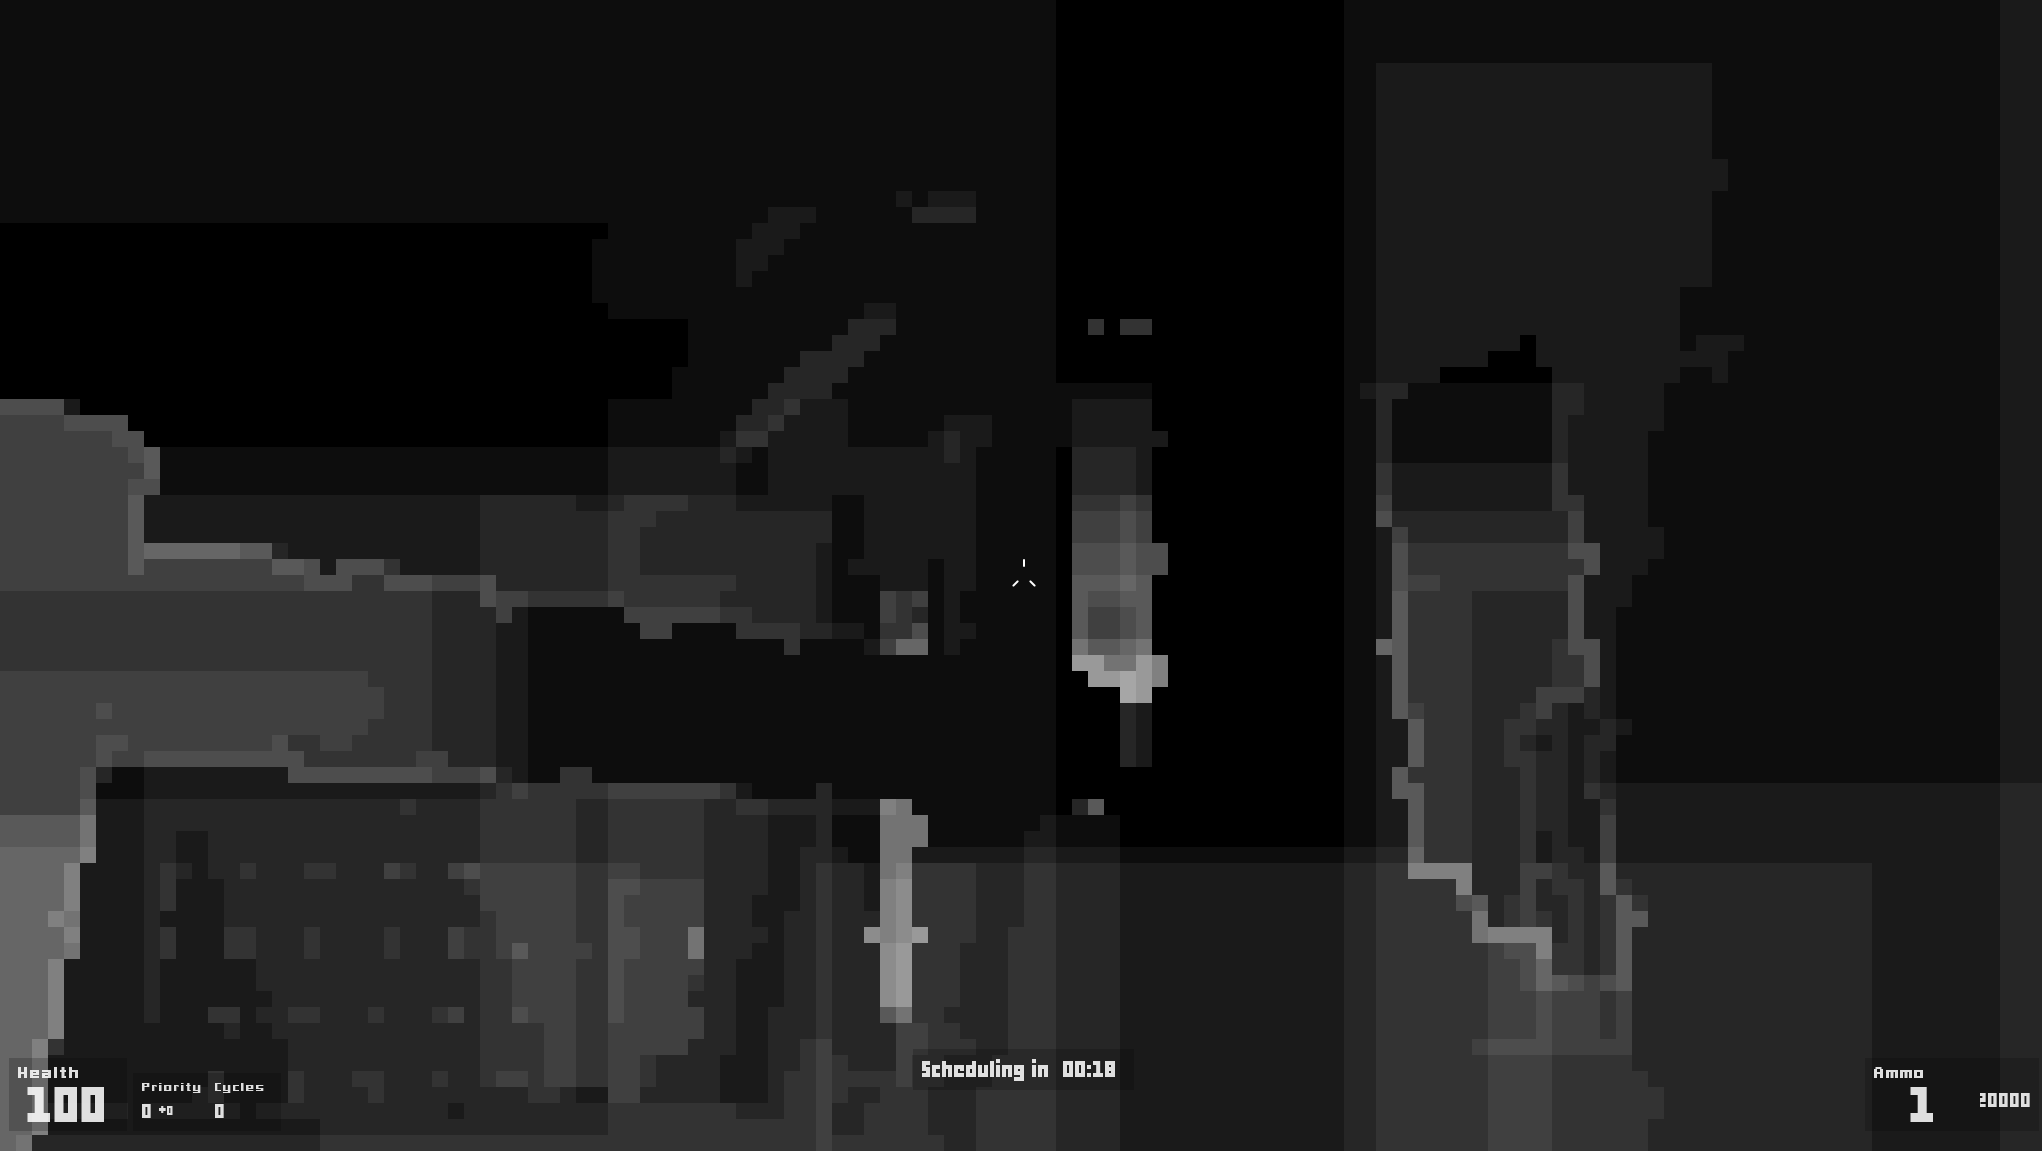
\includegraphics[width=1.0\textwidth]{img/tbds1.png}
  \end{minipage}
  \hspace{0.25cm}
  \begin{minipage}[b]{0.3\linewidth}
    \centering
    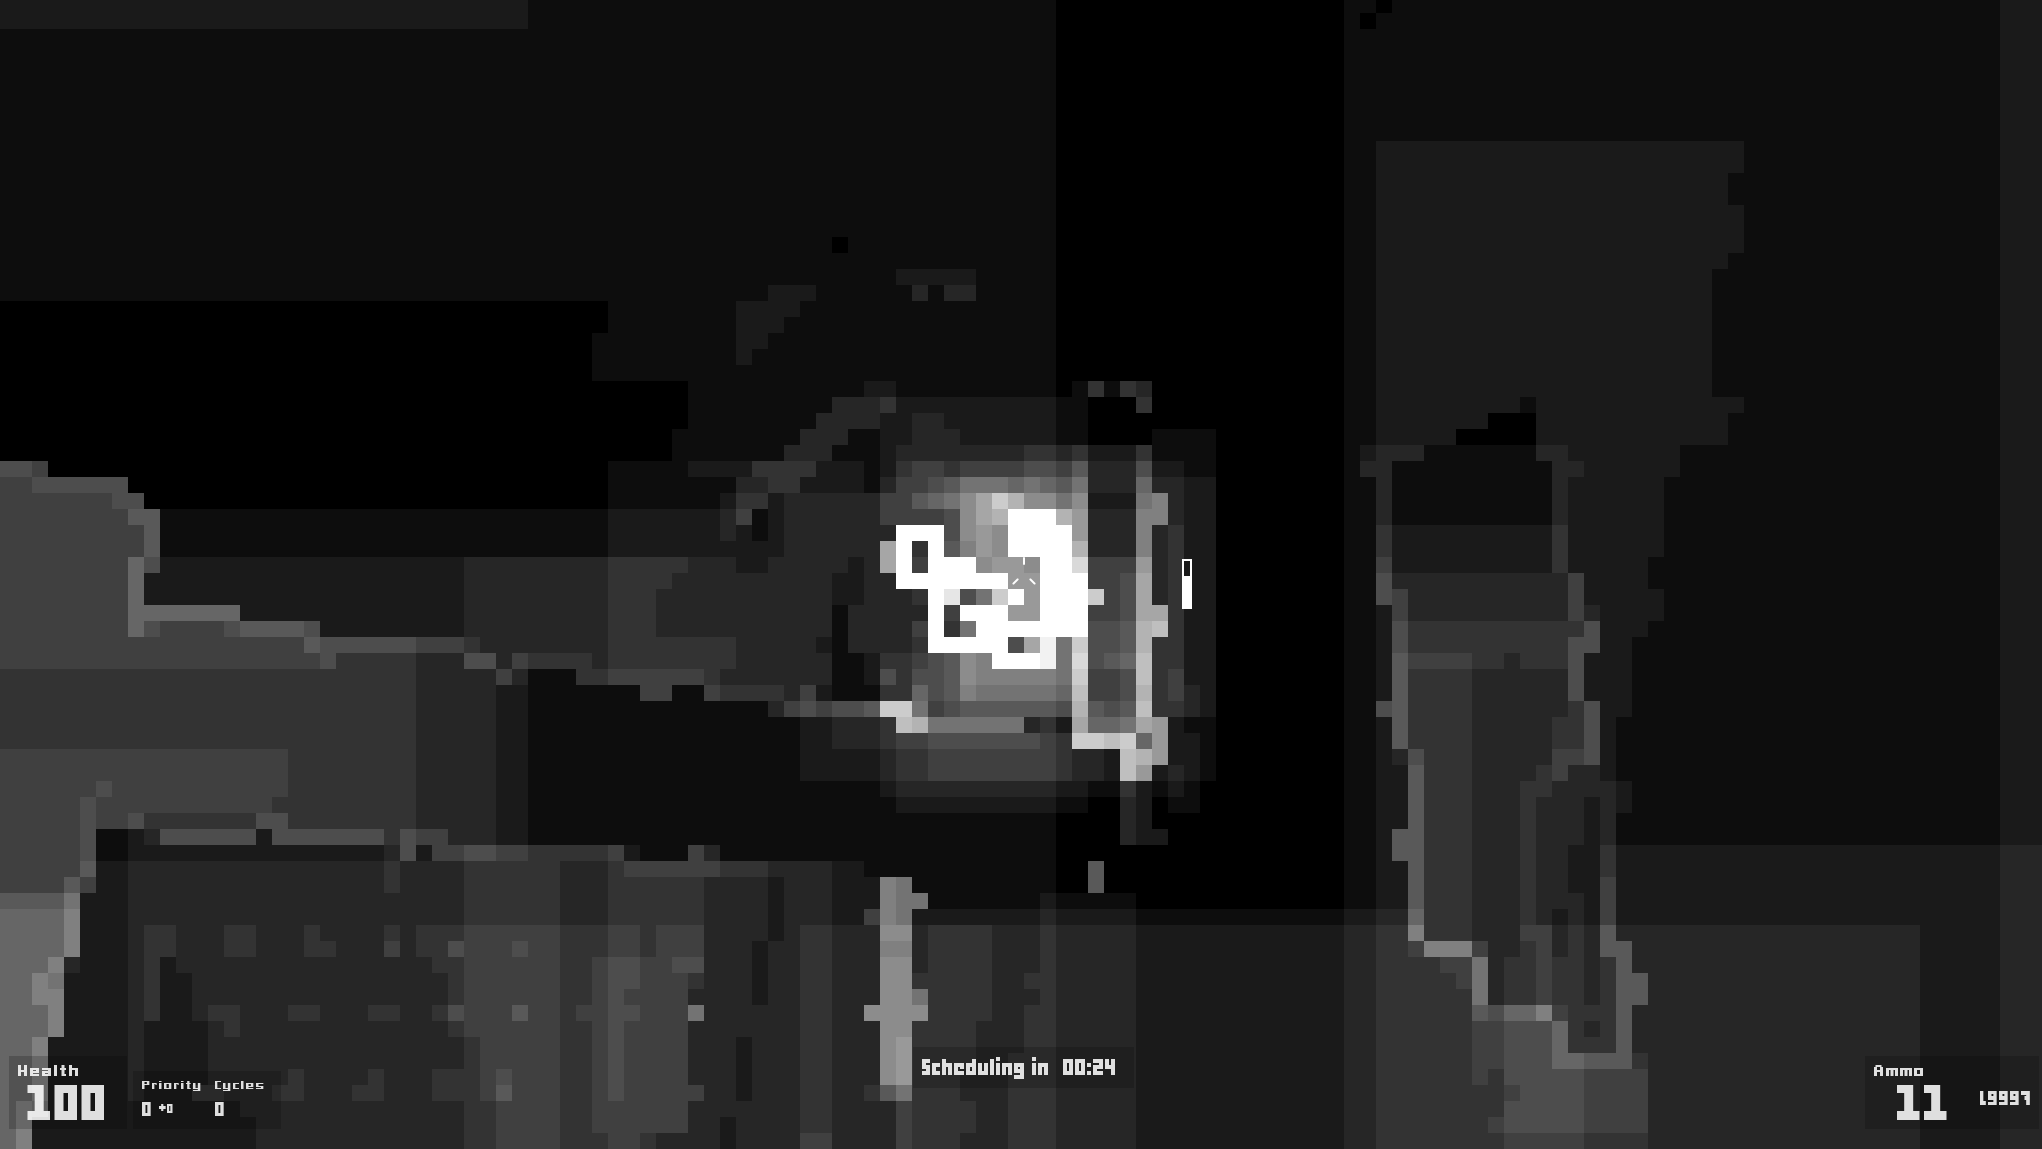
\includegraphics[width=1.0\textwidth]{img/tbds2.png}
  \end{minipage}
  \hspace{0.25cm}
  \begin{minipage}[b]{0.3\linewidth}
    \centering
    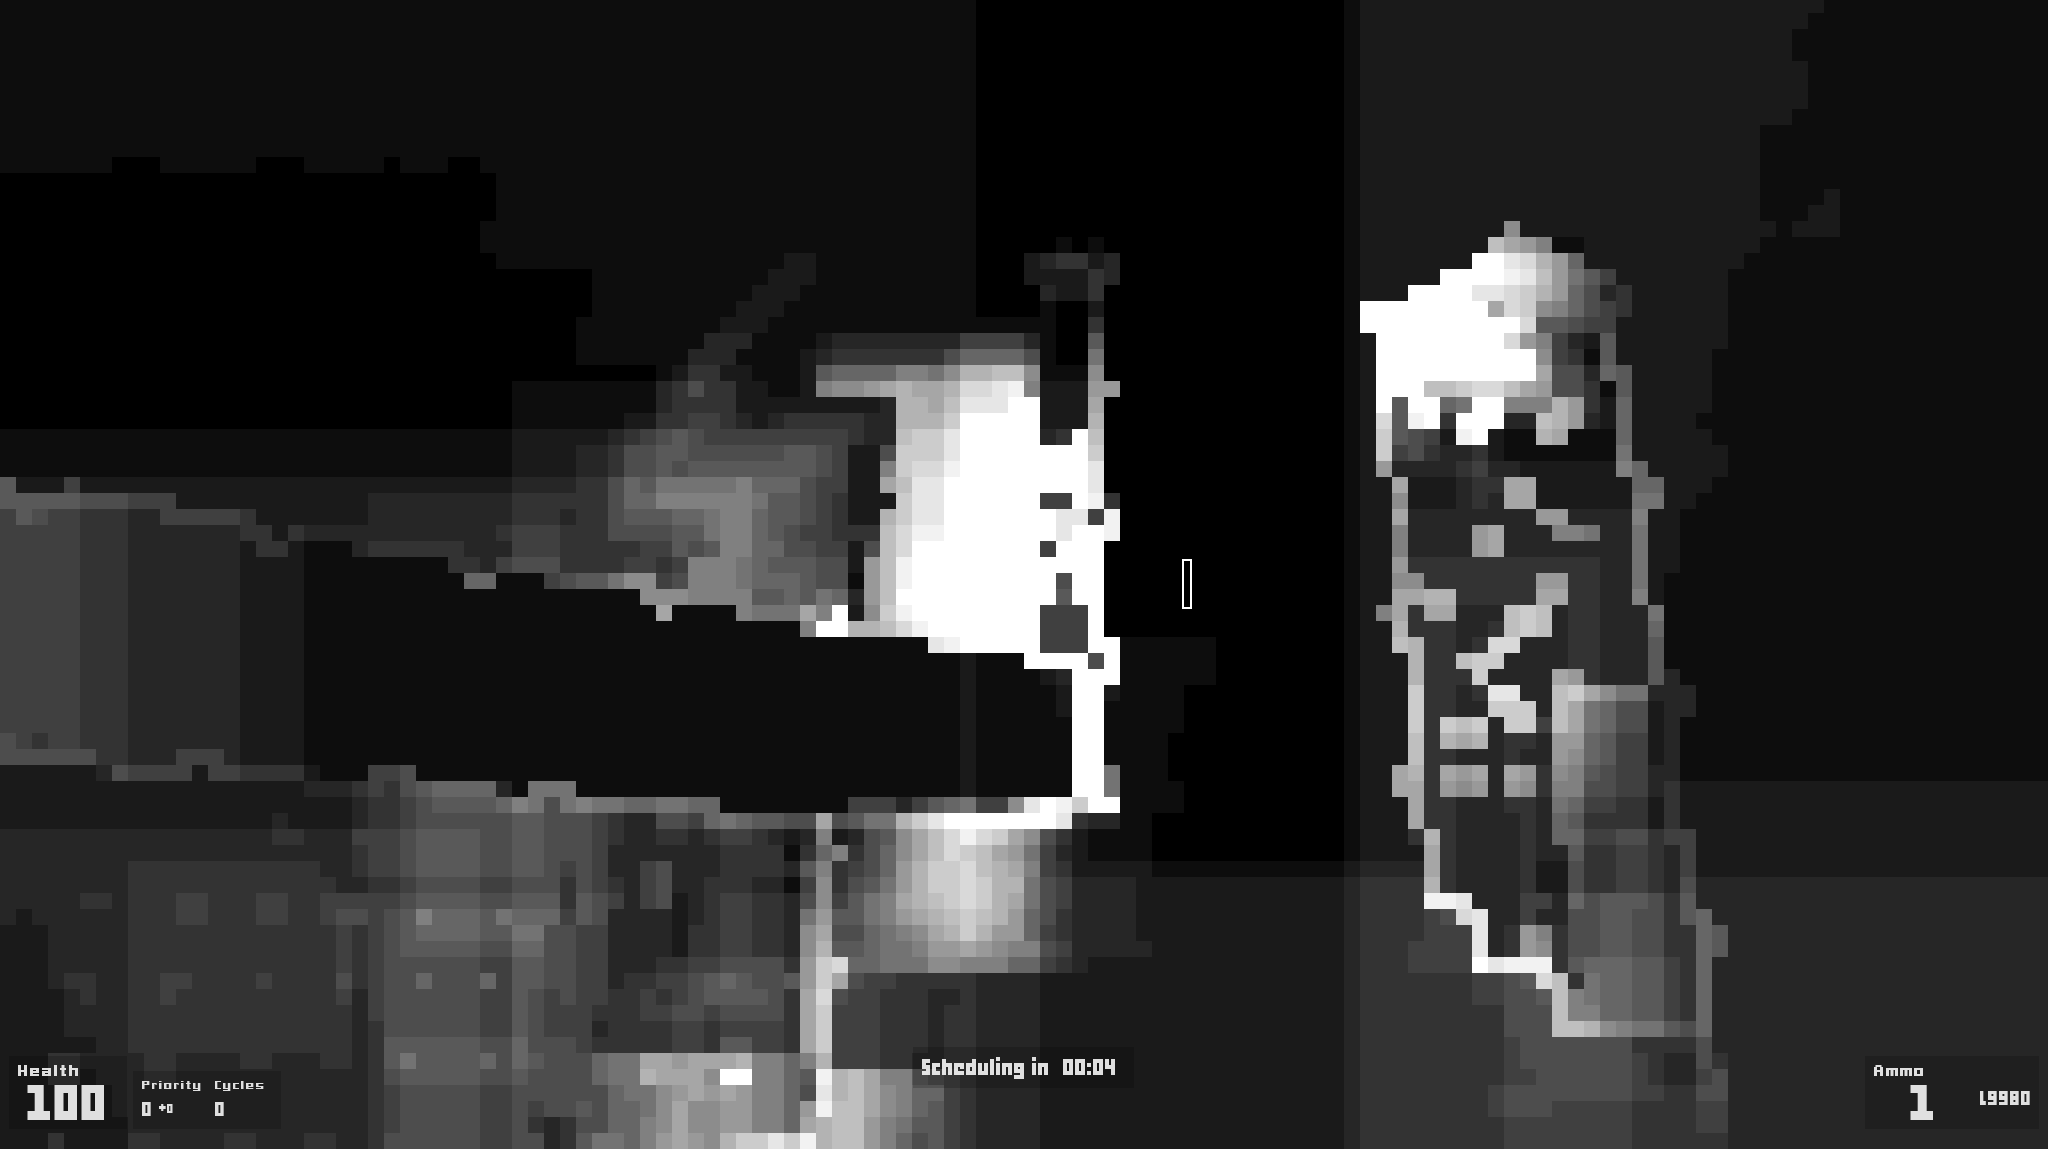
\includegraphics[width=1.0\textwidth]{img/tbds3.png}
  \end{minipage}
  \label{fig:tilingvisualization}
  \caption{Tile-based deferred shading using DirectCompute.}
\end{figure}

\begin{figure}[ht]
  \begin{minipage}[b]{0.3\linewidth}
    \centering
    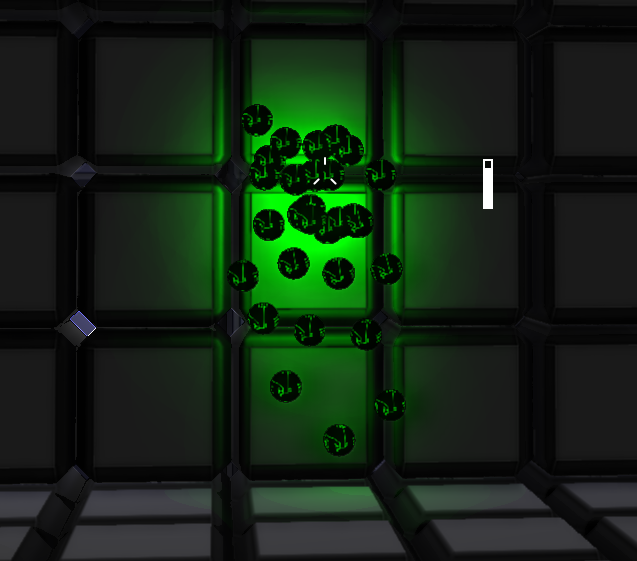
\includegraphics[width=1.0\textwidth]{img/tbds.png}
    \caption{AMD}
  \end{minipage}
  \hspace{0.25cm}
  \begin{minipage}[b]{0.3\linewidth}
    \centering
    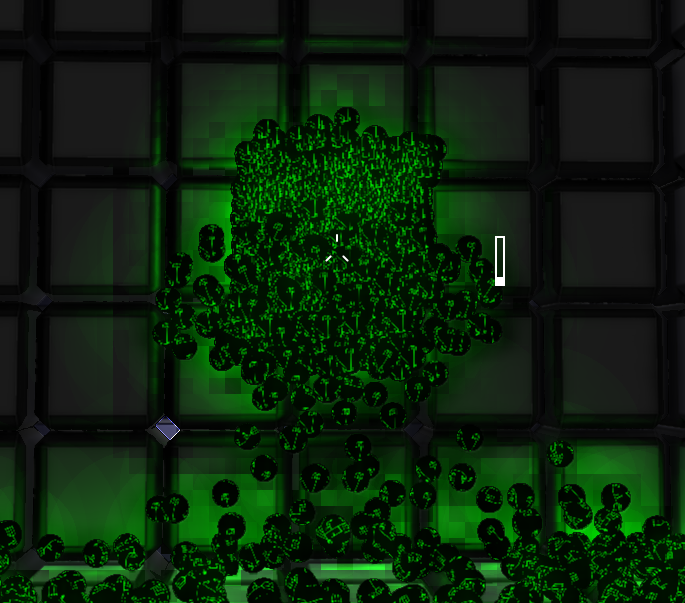
\includegraphics[width=1.0\textwidth]{img/tbds_error.png}
    \caption{NVIDIA\textit{*≠}}
  \end{minipage}
  \label{fig:tilingerror}
\end{figure}

\end{frame}

% WARP
\subsection{Microsoft WARP}
\begin{frame}
\frametitle{MICROSOFT WARP}

Introductory frame on Microsoft WARP.

\end{frame}
